\chapter{Praktische Evaluation}

\section{Experimentelle Umgebung}
Die folgenden Experimente wurden auf Rechner mit Ubuntu 24.04 und einem AMD EPYC 7763 CPU mit 16 nutzbaren Hardwarethreads durchgeführt. Die C++-Implementierung wurde
mithilfe von GCC in der Version 13.2.0 kompiliert.

\section{Implementierung}
Die Implementierung der Algorithmen erfolgte im C++20-Standard.

\section{Daten}
Die Experimente wurden auf verschiedenen Datenbausteinen vom Pizza \& Chili-Corpus durchgeführt. Die verwendeten Datenbausteine sind in der folgenden Tabelle aufgelistet.

\begin{figure}
    \centering
    \caption{Auflistung der verwendeten Eingabedaten auf dem Pizza \& Chili-Corpus. Neben der Bezeichnung der Datei ist die Dateigröße, die Größe des Alphabets, sowie eine kurze 
    Beschreibung des Inhalts angegeben}
    \begin{tabular}{|c|c|c|c|c|}
        \hline
        \textbf{Datei} & \textbf{Größe} & \textbf{Alphabet} & \textbf{Beschreibung} \\
        \hline
        \hline
        \texttt{dna} & 100MB & 4 & DNA-Sequenzen \\
        \hline
        \texttt{english} & 100MB & 256 & Englische Texte \\
        \hline
        \texttt{proteins} & 100MB & 20 & Proteinsequenzen \\
        \hline
        \texttt{sources} & 100MB & 256 & Quellcode \\
        \hline
        \texttt{xml} & 100MB & 256 & XML-Dateien \\
        \hline
    \end{tabular}
\end{figure}

\section{Ergebnisse}
Die Ergebnisse der Experimente sind in den folgenden Tabellen und Abbildungen dargestellt.

\begin{figure}
\centering
\caption{Laufzeit der Algorithmen auf Präfixen verschiedener Größen der Datei Proteins}
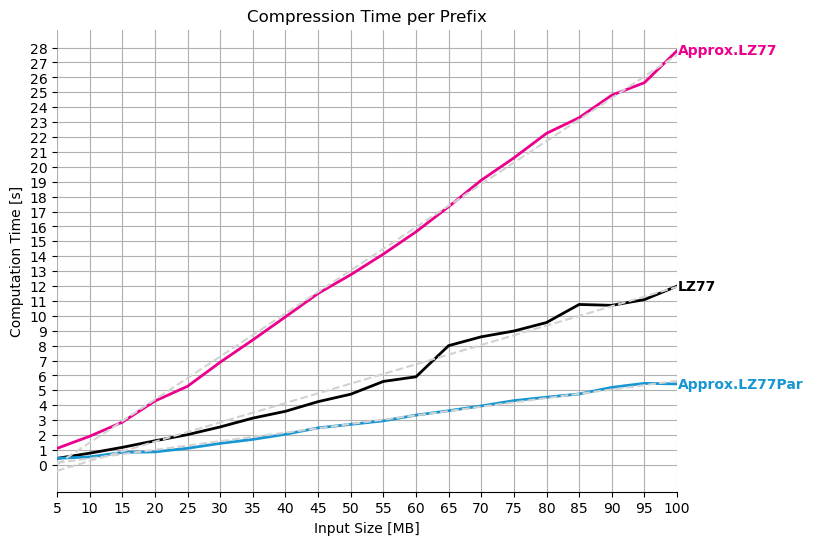
\includegraphics[scale=0.6]{bilder/progressive.png}
\end{figure}

\begin{figure}
    \centering
    \caption{Laufzeit der parallelel Approximation von LZ77 mit verschiedenen Anzahlen von Threads}
    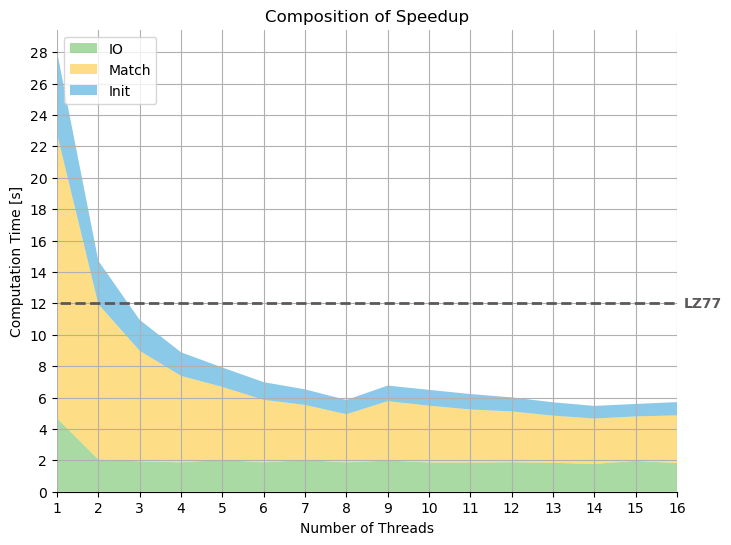
\includegraphics[scale=0.6]{bilder/progressive_speedup_stack.png}
\end{figure}